\section{Результат}

Результатом дипломной работы стал web-сервис для работы с трехмерными объектами.
Сервис предоставляет функционал по обработке трехмерных объектов, а именно:
\begin{itemize}
    \item Загрузку трехмерных моделей в формате *.OBJ
    \item Просмотр трехмерных моделей с функциями поворота, масштабирования
    и режимом автоматического вращения
    \item Локальное изменение трехмерных моделей с помощью специального инструмента
    \item Изменение трехмерных моделей за счет алгоритмов,
    реализованных на стороне сервера на языке С++
\end{itemize}

Разработанный сервис предоставляет следующие возможности модульного
расширения:
\begin{enumerate}
    \item Возможность добавления инструментов для взаимодействия с
    трехмерным объектом
    \item Возможность добавления алгоритмов на языке С++ для серверной обработки
    геометрии
\end{enumerate}

\begin{figure}[htb]
\centering
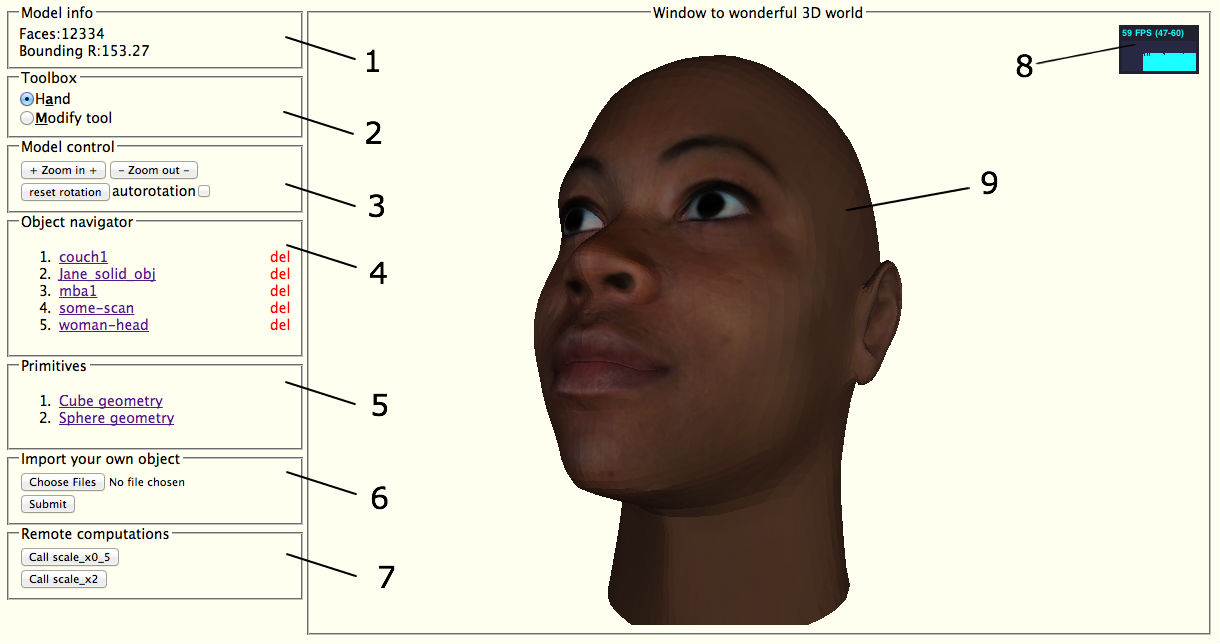
\includegraphics[width=1.0\textwidth]{ui.jpg}
\caption{Интерфейс приложения}
\label{fig:ui}
\end{figure}

На рисунке ~\ref{fig:ui} представлен внешний вид клиентской части разработанного
клиент-серверного приложения
\begin{description}
    \item[1 Информация] Здесь предоставляется информация о количестве
    полигонов и радиусе описанной окружности модели.
    \item[2 Инструменты] Набор инструментов для
    взаимодействия с моделью. Для выбора возможно использование быстрых клавиш
    \item[3 Управление моделью] Управление объектом: приближение, удаление,
    автоматическое вращение объекта
    \item[4 Инспектор объектов] База преобразованных OBJ-файлов, доступных для
    динамической загрузки в редактор. Нажатие ссылки ``del'' рядом с каждым объектом
    приведет к его удалению из базы.
    \item[5 Графические примитивы] Загрузка графических примитивов в поле
    редактора
    \item[6 Импорт OBJ-объектов] Форма для добавления OBJ-объектов в инспектор
    объектов.
    \item[7 Серверные вычисления] Список доступных функций преобразования
    геометрии, заданных и выполняемых на стороне сервера
    \item[8 FPS гистограмма] Статистика по количеству FPS
    \item[9 3D сцена] Сцена с трехмерным объектом
\end{description}
